\section {Rastreamento}	

	Rastreamento de objetos é uma importante tarefa do campo da computação visual. A proliferação de computadores com um alto poder computacional, a disponibilidade de câmeras de alta qualidade e preço acessível e a crescente necessidade de sistemas automáticos de análise de vídeos têm gerado um grande interesse em algoritmos de rastreamento de objetos~\cite{yilmaz}.

	Basicamente, rastreamento pode ser definido como o problema de estimar a trajetória de um objeto em um plano de imagem a medida em que se move na cena. Em outras palavras, um rastreador atribui \textit{labels} para os objetos monitorados em diferentes quadros de um vídeo~\cite{yilmaz}.

	A detecção e o rastreamento de pessoas tem um grande potencial em aplicações em domínios tão diversos como animação, interação humano-computador, vigilância automatizada (monitorar uma cena para detectar atividades suspeitas), entre outros. Por esta razão, tem havido um crescimento notável na investigação deste problema.

	O rastreamento de pessoas em um ambiente é considerada como uma tarefa complexa devido a:

		\begin{enumerate}
			\item complexidade do corpo humano;
			\item alta dinamicidade do ambiente;
			\item ruído nas imagens~\cite{yilmaz};
			\item complexidade do movimento das pessoas;
			\item oclusões parciais ou totais de pessoas;
			\item variação na iluminação do ambiente~\cite{yilmaz};
			\item processamento em tempo-real~\cite{yilmaz};
		\end{enumerate}

	Algumas dessas dificuldades podem ser vencidas com a utilização de imagens de profundidade ao invés de imagens de cor ou intensidade. As imagens de profundidade, além de serem muito pouco sensíveis as variações de iluminação, provê um fácil entendimento da estrutura da cena, que pode ser utilizada para simplificar as tarefas de rastreamento. Além disso, as câmeras que provêm imagens de profundidade estão comercialmente disponíveis a um preço acessível~\cite{nikos}.

	Várias abordagens para rastreamento de objetos já foram propostas. Basicamente, elas se diferem na forma que tratam as seguintes perguntas~\cite{yilmaz}: 
		
		\begin{itemize}
			\item Qual representação do objeto é adequada para o rastreamento?
			\item Quais características na imagem devem ser utilizadas?
			\item Como o movimento, aparência e a forma do objeto deve ser modelada? 
		\end{itemize}

	As respostas para estas perguntas dependem do contexto/ambiente onde o rastreamento será utilizado e do uso final para o qual as informações de rastreamento~\cite{yilmaz}.

	O rastreamento de pessoas geralmente inicia com o processo de segmentação da imagem da pessoa do resto da imagem. Depois, essas imagens segmentadas são transformadas em outras representações para reduzir a quantidade de informação ou para atender a um determinado algoritmo. Com isso, deve-se definir como as pessoas vão ser rastreadas \textit{frame} a \textit{frame}~\cite{moeslund}.

	Basicamente, o processo de rastreamento pode ser dividido em duas etapas:

		\begin{enumerate}
			\item Detecção do objeto;
			\item Rastreamento do objeto detectado;
		\end{enumerate}

	Antes de falarmos mais sobre cada uma dessas etapas e os métodos existentes para cada, vamos falar sobre as maneiras existentes de representar os objetos rastreados e sobre as características nas imagens que podem ser utilizadas.

%%%%%%%%%%%%%%%%%%%%%%%%%%%%%%%%%%%%%%%%%%%%%%%%%%%%%%%%%%%%%%%%%%%%%%%%%%%%%%%%%%%%%%%%%%%%%%%%%%%%%%%%%%%%%%%%%%%%%%%%%%%%%%%%%%%%%%%%%%%%%%%%%%%%%%%%%%%%%%%%%%%%%%%%%%%%%%%%%%%%%%%%%%%%%%%%%%%%%%%%%%%%%%%%%%%%%%%%%%%%%%%%%%%%%%%%%%%%%%%%%%%%%%%%%%%%%%%%%%%%%%%%%%%%%%%%%%%%%%%%%%%%%%%%%%%%%%%%%%%%%%%%%%%%%%%%%%%%%%%%%%%%%%%%%%%%%%%%%%%%%%%%%%%%%%%%%%%%%%%%%%%%%%%%%%%%%%%%%%%%%%%%%%%%%%%%%%%%%%%%%%%%%%%% 

\subsection{Representação do Objeto}

	Nos sistemas de rastreamento, os objetos rastreados devem ser representados de alguma maneira. Geralmente, as representações são baseados em suas formas. Existe uma forte relação entre a representação do objeto e o algoritmo de rastreamento escolhido~\cite{yilmaz}. A representação é escolhida baseada no domínio da aplicação e as mais utilizadas são:

	\begin{figure}[hbt]
		\begin{center}
			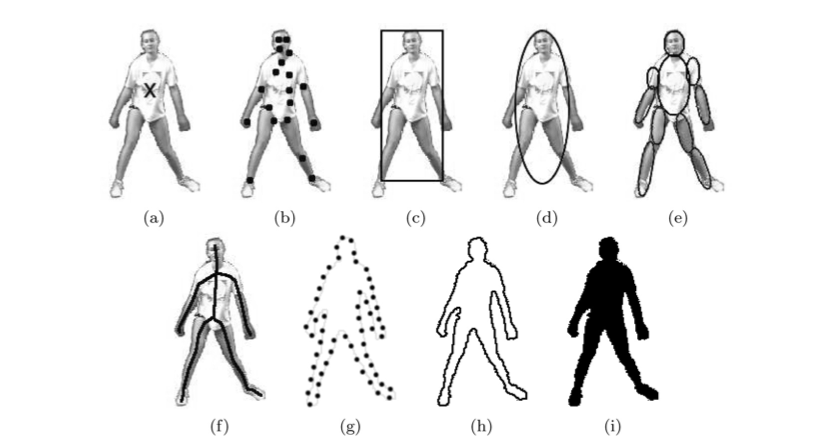
\includegraphics[scale=0.5]{figuras/2.FundamentacaoTeorica/representacao.png}
		\end{center}
		\caption{Representações de objetos rastreados. (a) Centroide, (b) múltiplos pontos, (c) representação retangular, (d) representação elíptica, (e) representação de múltiplas partes, (f) esqueleto do objeto, , (g) contorno completo do objeto, (h) contorno do objeto por pontos, (i) silhueta do objeto~\cite{yilmaz}}
		\label{representacao}
	\end{figure}

	\begin{itemize}
		\item \textbf{Pontos:} o objeto é representado por um ponto, como por exemplo a centroide da Figura \ref{representação}(a), ou por vários pontos, como por exemplo na Figura \ref{representacao}(b). Essa representação é mais adequada para rastreamento de objetos que ocupam uma pequena região na imagem~\cite{yilmaz};

		\item \textbf{Formas geométricas primitivas:} o objeto é representado por formas geométricas simples como um retângulo ou uma elipse, como mostrados nas Figuras \ref{representacao}(c) e (d). Essa representação é mais adequada para simples objetos rígidos~\cite{yilmaz};

		\item \textbf{Silhueta e Contorno:} representação por contorno define os limites de um objeto, como mostrado nas Figura \ref{representacao}(g) e (h). A região interna do contorno é chamada de Silhueta, como mostrado na Figura \ref{representacao}(i). Essa representação é mais adequada para rastrear objetos complexos de forma não rígida~\cite{yilmaz}. Ela é popular devido a sua simplicidade. A silhueta ou contorno de um objeto pode ser obtida definindo métodos de limiarização ou subtração, podendo ser utilizada tanto com imagens 2D quanto 3D. A representação 2D geralmente é mais simples~\cite{moeslund};

		\item \textbf{Modelos de formas articuladas:} objetos articulados são compostos por partes do corpo que se ligam por meio de juntas. Para representar objetos articulados, utiliza-se figuras geométricas para cada parte do corpo, como mostrado na Figura \ref{representacao}(e)~\cite{yilmaz};

		\item \textbf{Modelos de Esqueletos:} modelos de esqueletos são extraídos do objeto rastreado, como mostrado na Figura \ref{representacao}(f). Essa representação pode ser utilizada tanto para objetos articulados rígidos quanto não rígidos~\cite{yilmaz};
	\end{itemize}

	Para rastreamento de pessoas a representação por meio de contorno ou silhuetas são as mais adequadas~\cite{yilmaz}.

	O rastreamento de várias pessoas de maneira simultânea é considerada uma tarefa muito complexa. As representações das pessoas rastreadas podem se dividir ou fundir em novas representações devido a possíveis oclusões ou ruídos na imagem, e a aparência do objeto pode variar devido a sombras e mudanças da iluminação~\cite{moeslund}.

%%%%%%%%%%%%%%%%%%%%%%%%%%%%%%%%%%%%%%%%%%%%%%%%%%%%%%%%%%%%%%%%%%%%%%%%%%%%%%%%%%%%%%%%%%%%%%%%%%%%%%%%%%%%%%%%%%%%%%%%%%%%%%%%%%%%%%%%%%%%%%%%%%%%%%%%%%%%%%%%%%%%%%%%%%%%%%%%%%%%%%%%%%%%%%%%%%%%%%%%%%%%%%%%%%%%%%%%%%%%%%%%%%%%%%%%%%%%%%%%%%%%%%%%%%%%%%%%%%%%%%%%%%%%%%%%%%%%%%%%%%%%%%%%%%%%%%%%%%%%%%%%%%%%%%%%%%%%%%%%%%%%%%%%%%%%%%%%%%%%%%%%%%%%%%%%%%%%%%%%%%%%%%%%%%%%%%%%%%%%%%%%%%%%%%%%%%%%%%%%%%%%%%%%

\subsection{Características para rastreamento}

	A seleção das características é uma tarefa crítica para o rastreamento e está fortemente relacionada com a representação do objeto. Em geral, a seleção procura as características mais singulares para que o objeto rastreado seja facilmente distinguido~\cite{yilmaz}. As características mais comuns utilizadas atualmente são:

	\begin{itemize}
		\item \textbf{Cor:} a cor do objeto é influenciada principalmente por duas características: a distribuição da iluminação e a propriedade de reflectância do objeto. Geralmente, a representação \textit{RGB} é utilizada para representar a cor~\cite{yilmaz};

		\item \textbf{Borda:} os limites de um objeto geram uma grande variação na intensidade na imagem e são menos sensíveis a variações na iluminação comparado com as cores. A detecção por meio das bordas é utilizada para identificar essas variações de intensidade na imagem. Os algoritmos que detectam as bordas do objeto geralmente as utiliza para representação do mesmo~\cite{yilmaz};

		\item \textbf{Fluxo Óptico:} é um campo denso de vetores de deslocamento que define a tradução de cada pixel em uma região. Ele é calculado a partir da restrição de luminosidade, que pressupõe a constância de brilho de \textit{pixels} correspondentes nas \textit{frames} consecutivas~\cite{yilmaz};

		\item \textbf{Textura:} é a medida da intensidade da variação da superfície que quantifica propriedades como suavidade e regularidade. A Textura é menos sensível a variação da iluminação comparado com a cor~\cite{yilmaz};

	\end{itemize}

De todas as características, a mais utilizada para rastreamento é a cor~\cite{yilmaz}.

\subsection{Detecção de objeto}

	Todo método de rastreamento requer um mecanismo de detecção de objetos que pode ser realizada a cada \textit{frame} obtida ou na primeira vez que o objeto aparece no vídeo. Os método mais populares são:


	\begin{itemize}
		\item \textbf{Detector de pontos:} esses detectores são usados para encontrar pontos de interesses dentro da imagem que tem uma expressiva textura na sua respectiva localização. Pontos de interesse são amplamente usados no contexto do movimento e no rastreamento. A qualidade desejável para o ponto de interesse é que seja invariante diante das mudanças de iluminação e ângulo de visão da câmera~\cite{yilmaz}.
	
		\item \textbf{Subtração de fundo:} é um método popular para segmentação de movimento, especialmente nas situações em que o plano de fundo é relativamente estático. Ele detecta as regiões de movimento na imagem obtendo a diferença pixel a pixel entre a \textit{frame} corrente e a \textit{frame} referente ao plano de fundo~\cite{weiming}. Geralmente, um algoritmo de componentes conectadas é aplicado para obter regiões conectadas que correspondem a um objeto~\cite{yilmaz}.

		\item \textbf{Segmentação:} o objetivo do algoritmo de segmentação é particionar a imagem em regiões com certo grau de similaridade. Todo algoritmo de segmentação tem dois problemas: o critério para definir uma boa partição e o método para arquivar particionamentos eficientes~\cite{yilmaz}.

		\item \textbf{Aprendizagem supervisionada:} a detecção de objetos pode ser feita pelo aprendizado automático de diferentes objetos de um conjunto de exemplos por meio de um mecanismo de aprendizado. Esse aprendizado requer o armazenamento de um um conjunto de \textit{templates}. A partir desse conjunto de informações, o algoritmo gera uma função que mapeia as possíveis entradas para as saídas desejadas. Um problema padrão é a classificação onde a função gera um valor contínuo a partir de um determinado comportamento do objeto. No contexto da detecção de objetos as informações armazenadas são compostas por um par de características de objetos e uma classe associada onde ambos os valores são manualmente definidos. Seleção de características tem um papel importante no desempenho da classificação, portanto, é importante usar um conjunto de características que seja possível discriminar uma classe das outras~\cite{yilmaz}.
	\end{itemize}


\subsection{Rastreamento de objeto}

	O objetivo do rastreamento de objeto é conhecer a trajetória do mesmo no tempo localizando sua posição em cada \textit{frame}. O rastreamento de objetos também pode prover a região completa na imagem ocupada pelo objeto a cada instante~\cite{yilmaz}. 

	As atividades de detecção de objetos e de estabelecimento de correspondências entre a objetos e as instâncias dos \textit{frames} podem ser realizadas tanto separadamente como concomitantemente. No primeiro caso, as prováveis regiões de objetos são obtidas e o rastreador encontra correspondência entre os objetos e os \textit{frame}s. No último caso, as prováveis regiões e as correspondências são feitas juntas e estimadas pela atualização iterativa da localização do objeto e de regiões de informações obtidos dos \textit{frames} anteriores~\cite{yilmaz}.

	Os métodos de rastreamento de objetos mais utilizados atualmente são:

	\begin{itemize}
		\item \textbf{Rastreamento de pontos:} os objetos detectados a cada frame são representados por pontos e a associação entre os pontos é feita com base no estados anterior do objeto que pode incluir a posição e o movimento. Essa abordagem requer um mecanismo externo para detectar o objeto a cada \textit{frame}~\cite{yilmaz};

		\item \textbf{Rastreamento de \textit{kernel}}: os objetos são rastreados pelo cálculo do movimento do \textit{kernel} em \textit{frames} consecutivas. Esse movimento geralmente esta na forma de transformações paramétricas como translação e rotação. \textit{Kernel} se refere ao formato ou aparência do objeto~\cite{yilmaz}.

		\item \textbf{Rastreamento de Silhuetas:} o rastreamento é feito estimando a região do objeto a cada \textit{frame}. Esse método utiliza informação contida dentro da região do objeto. Esta informação pode ser na forma de densidade de aparência e modelos de forma que estão, geralmente, na forma de mapas borda. Dado os modelos de objeto, silhuetas são rastreadas por qualquer forma de correspondência ou evolução de contorno. Ambos os métodos podem ser essencialmente considerados como segmentação de objetos aplicada no domínio temporal utilizando os priores gerados a partir dos \textit{frames} anteriores~\cite{yilmaz}.
	\end{itemize}




